\chapter[Scaling Partitioned Replicated System]{Scaling Partitioned Replicated System}

Today's online services of all size enterprises must meet strict availability
and performance requirements, as part of their broader digital transformation
strategy. In order to meet the strict availability requirements, those online
services must be replicated. State machine replication is a fundamentally
powerful building block that enables the implementation of highly available
distributed services by replication. State machine replication achieves strong
consistency (i.e., linearizability) by regulating how client commands are
propagated to and executed by the replicas: every non-faulty replica must
receive and execute every command deterministically and in the same order. If
all replicas have to execute the same sequence of commands, the system can not
scale. Increasing the number of replicas results in bounded improvements in
performance.

Scalable performance can be achieved with state partitioning. Partitioning (also
known as \emph{sharding}) is a technique that divides the state of a service in
multiple partitions so that most commands access one partition only and are
equally distributed among partitions. Partitioning replicated state machine can
lead to highly scalable and available systems, however, introduce daunting
challenges. Most services cannot be ``perfectly partitioned", that is, the
service state cannot be divided in a way that commands access one partition
only. Therefore, a partitioning scheme must cope with multi-partition commands.

There are two general solutions to handle multi-partition commands in terms of
consistency guarantees. One solution, known as \textbf{weak consistency}, is to
weaken the guarantees of commands that involve multiple partitions (e.g.,
\cite{facebookTAO}). In the context of SMR, this would mean that requests access
data within single partition (single-partition commands) are strongly consistent
(i.e., linearizable), while concurrent requests accessing multiple partitions
(multi-partition commands) may lead to inconsistencies. This approach relaxes
the consistency guarantees and makes systems less exposed to impossibility
results \cite{FLP85, diskpaxos}, but makes the effects of data partitioning and
replication visible to the application. To lower the chance of potential
conflicts, data access patterns can be considered when partitioning data (e.g.,
objects often accessed together can be co-located in the same partition). But
these optimizations require prior knowledge about the workload, and are often
performed offline \cite{facebookTAO}

The other solution, known as \textbf{strong consistency}, is to
provide strong consistency guarantees for both single- and multi-partition
commands, at the cost of a more complex execution path for commands that involve
multiple partitions.


In the scope of this thesis, we only focus on the second
category, that is replicated state machine systems that provide strong
consistency.

Essentially, in a distributed system, there are two different ways to handle
commands:


\section{Scalability in distributed database system}

Sharding is a database architecture pattern related to horizontal partitioning —
the practice of separating one table’s rows into multiple different tables,
known as partitions. Each partition has the same schema and columns, but also
entirely different rows. Likewise, the data held in each is unique and
independent of the data held in other partitions. Sharding involves breaking up
one’s data into two or more smaller chunks, called logical shards. The logical
shards are then distributed across separate database nodes, referred to as
physical shards, which can hold multiple logical shards. Despite this, the data
held within all the shards collectively represent an entire logical dataset.
ç
Google Spanner~\cite{corbett2013spanner} was designed to be a highly-scalable
distributed relational database. Spanner consists of multiple \emph{zones}, each
of which is a deployment of Bigtable servers. A zone uses one \emph{zonemaster}
to assign data to one hundred to several thousand sets of Paxos-based state
machines (so called \emph{spanservers}).
% Clients in Spanner use \emph{location
% proxy} of each zone to locate the spanservers assigned to serve their data.
The steps to process a multi-partition transaction are the following. First, a
client communicates with a proxy location to determine which groups maintain the
data touched by the transaction. Second, the client retrieves this data from the
groups, acquiring locks for them. Next, the client executes its transaction
locally, chooses one of the groups involved in the transaction as a coordinator
group C, and sends the result and the id of C to all groups involved in the
transaction. Finally, group C coordinates a two-phase commit with the other
groups for committing the transaction

Although not detailed in the paper, Spanner allows data to be re-sharded across
\emph{spanservers} or \emph{zones} data centers to balance loads and in response
to failures by \emph{placement driver}. Periodically, \emph{placement driver}
communicates with spanservers to re-arrange data. During these transfers,
clients can still execute transactions (including updates) on the database.
Figure~\ref{fig:spanner} shows an execution of a single transactions that
requires multiple round of coordination in Spanner.

Distributed operators appear in execution plans with a distributed union variant
on top of one or more local distributed union variants. A distributed union
variant performs the remote distribution of subplans. A local distributed union
variant is on top of each of the scans performed for the query, as shown in the
execution plan in Figure~\ref{fig:spanner-plan}. The local distributed union
variants ensure stable query execution when restarts occur for dynamically
changing split boundaries. Whenever possible, a distributed union variant has a
split predicate that results in split pruning, meaning the remote servers
execute subplans on only the splits that satisfy the predicate. This improves
both latency and overall query performance.


\begin{figure*}
  \begin{minipage}[b]{1.0\linewidth}
  \centering
        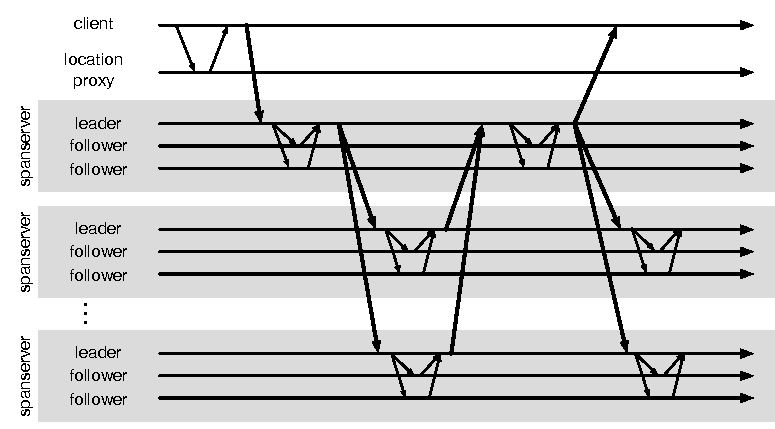
\includegraphics[width=0.6\linewidth]{figures/spanner-execution}
  \end{minipage}
  \caption{Coordination required in multi-partition transaction in Spanner}
  \label{fig:spanner}
\end{figure*}

\begin{figure*}
  \begin{minipage}[b]{1.0\linewidth}
  \centering
        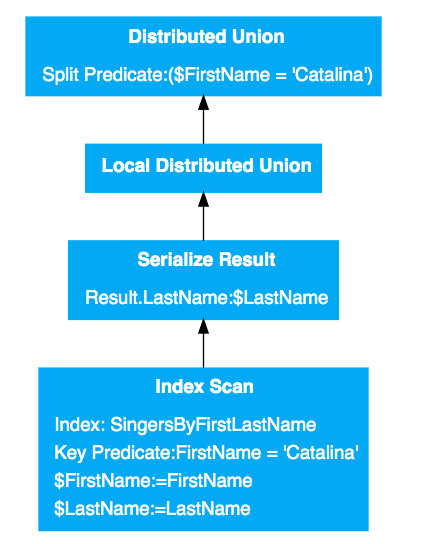
\includegraphics[width=0.6\linewidth]{figures/spanner-distributed-query}
  \end{minipage}
  \caption{Execution plan of a distributed query in Spanner}
  \label{fig:spanner-plan}
\end{figure*}


\section{Scaling state machine replication}

The classical SMR does not scale: adding resources (e.g., replicas) will not
translate into the improvement of performance, in terms of throughput. This
happens for a couple reasons. First, the underlying communication protocol
needed to ensure ordered message delivery may not scale itself (i.e., a
communication bottleneck). Second, every replica must execute the same sequence
of command to reach the same state (i.e., an execution bottleneck).

Several approaches have been proposed to address SMR's scalability limitations.
To cope with communication overhead, some proposals have suggested to spread the
load of ordering commands among multiple processes (e.g.,
\cite{Moraru:2013gw,Mencius,Marandi:2012hb}), as opposed to dedicating a single
process to determine the order of commands (e.g.,
\cite{Lam98}).%\fxnote[draft]{remove inapplicable reference}

Two directions of research have been suggested to overcome execution
bottlenecks. One approach (scaling up) is to take advantage of multiple cores to
execute commands concurrently without sacrificing consistency
\cite{Kapritsos:2012um,Marandi:2014bj,Kotla:2004ep,Guo:2014jp}. Another approach
(scaling out) is to partition the service's state and replicate each partition
(e.g., \cite{Glendenning:2011kj,Marandi:2011dj}). In this chapter, we review the
second category, which is be basic of our work.

\subsection{Partitioning application state}

Modern distributed systems typically scale performance by partitioning
application state and tolerate failures by replicating each partition. Clients
submit commands for execution to one or more partitions. Within a partition,
replicas coordinate by means of a consensus protocol (e.g., Paxos~\cite{Lam98}).
To coordinate the execution of multi-partition commands, replicated partitions
rely on some distributed coordination protocol (e.g., two-phase locking
\cite{corbett2013spanner}, optimistic concurrency control \cite{Chang:2008},
atomic multicast \cite{bezerra2014ssmr}).

In principle, increasing the number of partitions should result in increased
system performance. However, if the execution of commands involves multiple
partitions, then performance can actually decrease, due to overhead from
ordering and coordinating commands across partitions to ensure strong
consistency. Different techniques have been proposed to handle commands that
access state in multiple partitions, but inherently multi-partition commands are
more expensive than single-partition commands. Moreover, if data is not
distributed carefully, then load imbalances can nullify the benefits of
partitioning. Thus, an ideal partitioning scheme is one that would both (i)
allow commands to be executed at a single partition only, and (ii) evenly
distribute data so that load is balanced among partitions. We refer to workloads
that can be partitioned in a way that satisfies these two properties as
exhibiting \emph{strong locality}. Conversely, workloads that cannot avoid
multi-partition commands with balanced load among partitions exhibit \emph{weak
locality}.

Broadly speaking, there are two classes of techniques for partitioning:
\emph{static} and \emph{dynamic}. Figure~\ref{fig:motivation} shows the result
of a motivating experiment that compares two representative systems, one of each
class. In the experiment, we measured the throughput and number of state moves
over time with two different workloads: one with strong locality and one with
weak locality. The workloads are inspired by the social network Twitter, in
which the network is modeled as a graph, and users can ``post'' messages. The
social graph was generated using a Zipfian distribution, where the Zipf
parameter was adjusted to alter the locality.  For brevity, we postpone the
details of the experimental setup until Section~\ref{sec:dynastar-experiments}.
\emph{Static} techniques choose an immutable assignment of application state
variables to partitions prior to executing commands. This techniques requires a
good understanding about the workload to avoids load imbalances and favors
single-partition commands.  Moreover, many online applications experience
variations in demand. These happen for a number of reasons. In social networks,
for example, some users may experience a surge increase in their number of
followers (e.g., new ``celebrities"); workload demand may shift along the hours
of the day and the days of the week; and unexpected (e.g., a video that goes
viral) or planned events (e.g., a new company starts trading in the stock
exchange) may lead to exceptional periods when requests increase significantly
higher than in normal periods. These challenges perhaps explain why most
approaches that extend SMR with state partitioning delegate the task of
partitioning the service state to the application designer. \emph{Dynamic}
techniques address the limitations of static techniques by adapting the
partitioning scheme as workloads change. For example, a dynamic technique can
move data ``on demand'' to maximize the number of single partition user
commands, while avoiding imbalances in the load of the partitions. The major
challenge in designing a dynamic scheme is determining how the system selects
the partition to which to move data.


\begin{figure*}[ht!]
  \centering
  \begin{subfigure}[b]{0.45\textwidth}
    \centering
    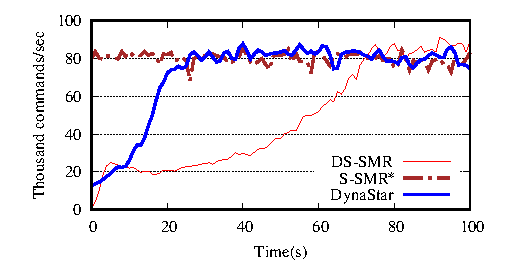
\includegraphics[width=0.95\columnwidth]{figures/experiments/dynastar/socc-tp-strong-locality}
    \caption{Throughput with strong locality}
  \end{subfigure}
  \begin{subfigure}[b]{0.45\textwidth}
    \centering
    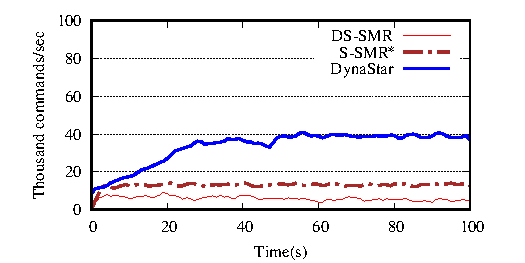
\includegraphics[width=0.95\columnwidth]{figures/experiments/dynastar/socc-tp-weak-locality}
    \caption{Throughput with weak locality}
  \end{subfigure} \\
  \begin{subfigure}[b]{0.45\textwidth}
    \centering
    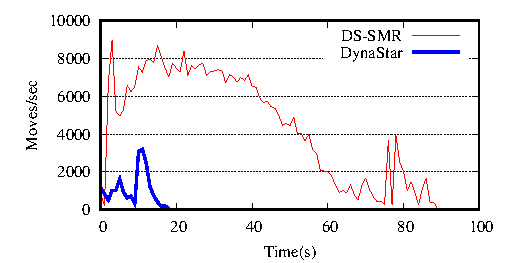
\includegraphics[width=0.95\columnwidth]{figures/experiments/dynastar/socc-moves-strong-locality}
  \caption{Number of move commands with strong locality}
  \end{subfigure}
  \begin{subfigure}[b]{0.45\textwidth}
    \centering
    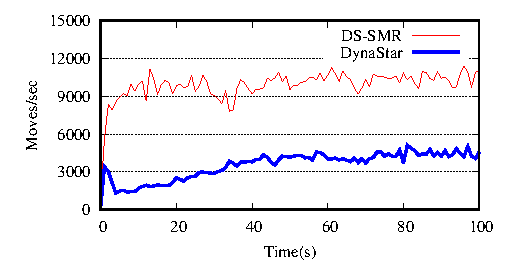
\includegraphics[width=0.95\columnwidth]{figures/experiments/dynastar/socc-moves-weak-locality}
    \caption{Number of move commands with weak locality}
  \end{subfigure}
  \caption{\dynastar, S-SMR* (i.e., optimized S-SMR) and DS-SMR under strong and weak locality, 4 partitions.}
  \label{fig:motivation}
\end{figure*}

\subsection{Static state partitioning with S-SMR}
\label{sec:ssmr}

In this section, we describe \ssmr\, an extension to SMR that under certain
workloads allows performance to grow proportionally to the number of replicas.
\ssmr\ partitions the service state and replicates each partition. It relies on
an atomic multicast primitive to consistently order commands within and across
partitions. In addition, \ssmr\ assumes a static workload partitioning. Any
state reorganization requires system shutdown and manual intervention.

In S-SMR~\cite{bezerra2014ssmr}, the service state \vvt\ is composed of $k$
partitions, in set $\Psi = \{\mathcal{V}_1, ..., \mathcal{V}_k\}$. Server group
$\ssm_i$ is assigned to partition $\mathcal{V}_i$. For brevity, we say that
server $s$ belongs to $\mathcal{V}_i$ meaning that $s \in \ssm_i$, and say
``multicast to $\mathcal{V}_i$'' meaning ``multicast to server group $\ssm_i$''.
S-SMR relies on an \emph{oracle}, which tells which partitions are accessed by
each command.

% \footnote{The oracle returns a set with the partitions accessed
% by the command, but this set does not need to be minimal; it may contain all
% partitions in the worst case, when the partitions accessed by the command cannot
% be determined before the command is executed.


\begin{figure*}
  \begin{minipage}[b]{1.0\linewidth}
  \centering
        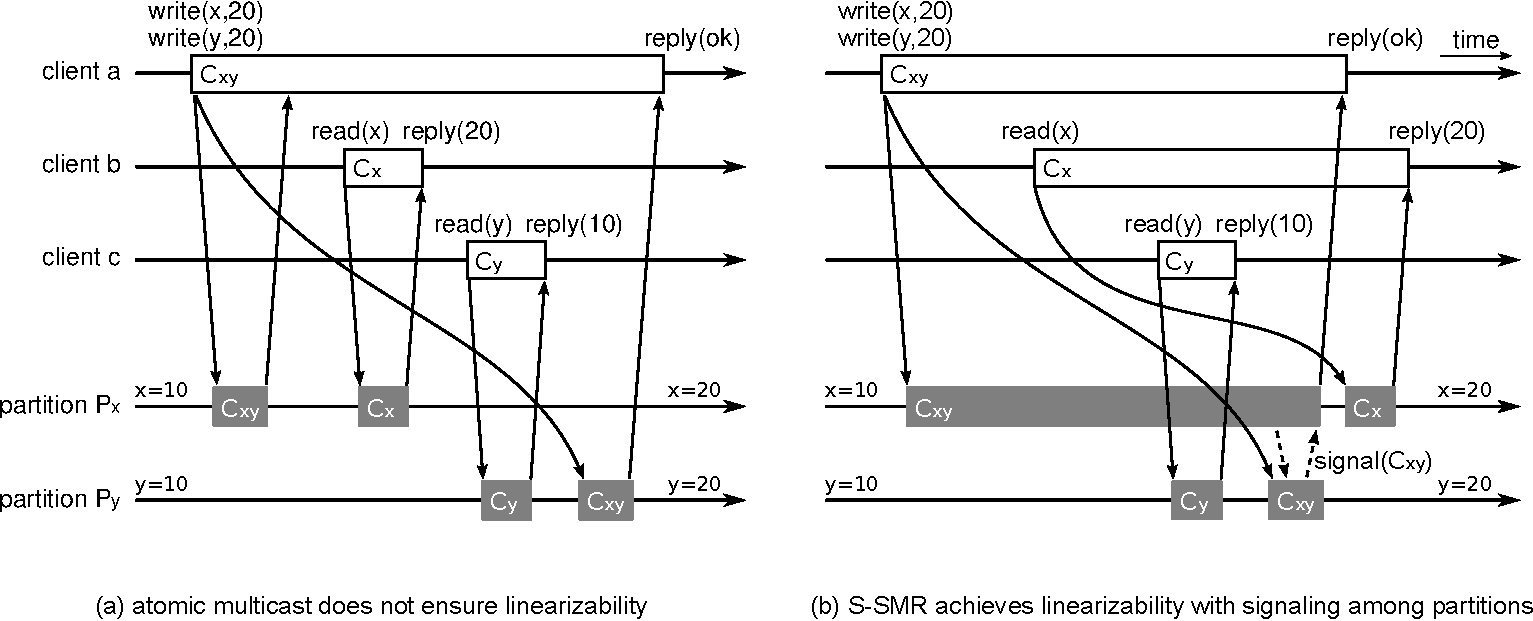
\includegraphics[width=1\linewidth]{figures/ssmr}
  \end{minipage}
  \caption{Atomic multicast and S-SMR. (To simplify the figure, we show a single replica per partition.)}
  \label{fig:ssmr}
\end{figure*}

To execute a command, the client multicasts the command to the appropriate
partitions, as determined by the oracle. Commands that access a single partition
are executed as in classical SMR: replicas of the concerned partition agree on
the execution order and each replica executes the command independently. In the
case of a multi-partition command, replicas of the involved partitions deliver
the command and then may need to exchange state in order to execute the command
since some partitions may not have all the values read in the command. This
mechanism allows commands to execute seamlessly despite the partitioned state.

S-SMR improves on classical SMR by allowing replicated systems to scale, while
ensuring linearizability. Under workloads with multi-partition commands,
however, it has limited performance, in terms of latency and throughput
scalability. Such decreased performance when executing multi-partition commands
is due to partitions (i) exchanging state variables and (ii) synchronizing by
exchanging signals. Thus, the performance of \ssmr\ is particularly
sensitive to the way the service state is partitioned.

One way to reduce the number of multi-partition commands is by dynamically
changing the partitioning, putting variables that are usually accessed together
in the same partition. However, the partitioning oracle of \ssmr\ relies on a
static mapping of variables to partitions. One advantage of this implementation
is that all clients and servers can have their own local oracle, which always
returns a correct set of partitions for every query. Such a static mapping has
the major limitation of not allowing the service to dynamically adapt to
different access patterns.

\subsection{Dynamic state partitioning}

%\ssmr\ performs better as the number of multi-partition commands decreases.




% Static techniques choose an immutable assignment of application state variables
% to partitions prior to executing commands. Dynamic techniques address the
% limitations of static techniques by adapting the partitioning scheme as
% workloads change. For example, a dynamic technique can move data ``on demand''
% to maximize the number of single partition user commands, while avoiding
% imbalances in the load of the partitions.
% %Typically, this is implemented by moving data ``on demand'' to a single
% %partition which executes a user command.
% The major challenge in designing a dynamic scheme is determining how the system
% selects the partition to which to move data.


% Figure~\ref{fig:motivation} shows the result of a motivating experiment that
% compares two representative systems, one of each class. In the experiment, we
% measured the throughput and number of state moves over time with two different
% workloads: one with strong locality and one with weak locality. The workloads
% are inspired by the social network Twitter, in which the network is modeled as a
% graph, and users can ``post'' messages. The social graph was generated using a
% Zipfian distribution, where the Zipf parameter was adjusted to alter the
% locality.  For brevity, we postpone the details of the experimental setup until
% Section~\ref{sec:experiments}.


% Static techniques choose an immutable assignment of application state variables
% to partitions prior to executing commands. As an example of a static approach
% for use in the experiment, we modified the S-SMR system~\cite{bezerra2014ssmr}
% to use the static METIS~\cite{Abou-Rjeili:2006} partitioning algorithm.  The
% METIS algorithm is optimized to minimize edge-cuts when partitioning a static
% social graph. In the workload with strong locality, METIS partitions the social
% graph such that all posts are single partition; in the workload with weak
% locality, although most commands are single partition, a small fraction of posts
% involves multiple partitions. The throughput is less for the weak locality
% workload due to the more expensive execution of multi-partition posts.
% %since the static scheme incurs overhead when accessing multiple partitions to
% %execute commands.
% For workloads that do not change the graph structure and exhibit strong
% locality, the results for optimized S-SMR in Figure~\ref{fig:motivation} show a
% theoretical maximum throughput.  Of course, these results are not achievable in
% practice, since for real workloads, the graph would change over time (e.g., in
% social networks users join and leave the system, connections are created and
% removed).


% Dynamic techniques address the limitations of static techniques by adapting the
% partitioning scheme as workloads change. For example, a dynamic technique can
% move data ``on demand'' to maximize the number of single partition user
% commands, while avoiding imbalances in the load of the partitions.
% %Typically, this is implemented by moving data ``on demand'' to a single
% %partition which executes a user command.
% The major challenge in designing a dynamic scheme is determining how the system
% selects the partition to which to move data.
% %
% The second system in Figure~\ref{fig:motivation} evaluates DS-SMR, a dynamic
% partitioning strategy implemented by  Le et al.~\cite{le2016dssmr}. This system
% selects partitions randomly, which allows for a completely decentralized
% implementation, in which partitions make only local choices about data movement.
% We refer to this approach as \emph{decentralized dynamic}.  As
% Figure~\ref{fig:motivation} shows, the decentralized dynamic approach works well
% for data with strong locality, but is unstable for workloads with weak locality,
% since data is constantly moved from one partition to another.



% \subsection{Scalable state-machine replication}
